
\section{Spannungstensor}

\paragraph{ Tensor:} 
	$ \left[\sigma_{ij}\right]
		=\left[\begin{matrix}
			\sigma_{xx} & \sigma_{yx} & \sigma_{zx} \\
			\sigma_{xy} & \sigma_{yy} & \sigma_{zy} \\
			\sigma_{xz} & \sigma_{yz} & \sigma_{zz}
		\end{matrix}\right]
	$

\paragraph{ Spannungsvektor:}
	$ \vec{\sigma}_n = \left[\sigma_{ij}\right]\cdot\vec{n} $
		\quad $ \sigma_{ni} = \sigma_{ij} n_j  $ 
		\qquad $ \vec{n} $ \dots muss Einheitsvektor sein
		
\paragraph{ Normalspannung:}
	$ \sigma_{nn} = \vec{\sigma}_n\cdot\vec{n} 
		= \left\{  [\sigma_{ij}] \cdot \vec{n}  \right\} \cdot \vec{n} $ 

\paragraph{ Schubspannung:}
	$ \tau = \sqrt{\sigma^2 - \sigma_n^2} 
		\quad \text{mit } \sigma = \absvec{\vec{\sigma}_{nn}}
		\qquad \vec{\tau} = \sigma_n - \sigma_{nn} \cdot \vec{n} 
		\quad  \rightarrow
		\quad \tau = \absvec{\vec{\tau}}
	$
	
\paragraph{ Hauptnormalspannungen:}
	$ 	- \sigma^3 + I_1 \cdot \sigma^2 - I_2 \cdot \sigma + I_3 = 0 $ \quad (Eigenwertproblem, lösen mit Rechenknecht)
	
\paragraph{ Koeffizienten (Invarianten) des Spannungstensors:}
	\[ 	I_1=\sigma_{xx}+\sigma_{yy}+\sigma_{zz}=\spur [\sigma_{ij}] \]
	\[ 	I_3=\det{\left[\sigma_{ij}\right]}=\sigma_1\cdot\sigma_2\cdot\sigma_3  \]
	\[ 	I_2 = 
		\begin{detmatrix}
			\sigma_{xx} & \sigma_{yx} \\
			\sigma_{xy} & \sigma_{yy}
		\end{detmatrix}
		+
		\begin{detmatrix}
			\sigma_{yy} & \sigma_{yz} \\
			\sigma_{yz} & \sigma_{zz}
		\end{detmatrix}
		+
		\begin{detmatrix}
			\sigma_{xx} & \sigma_{zx} \\
			\sigma_{xz} & \sigma_{zz}
		\end{detmatrix}
		=
		\sigma_1\cdot\sigma_2 + \sigma_2\cdot\sigma_3 + \sigma_3\cdot\sigma_1  
	\] 

\paragraph{ Normalrichtungen zu den Hauptnormalspannungen:}

	\[ 
	\left\{ \left[ \sigma_{ij} \right] - \sigma_i \cdot [I] \right\} \cdot \vec{n}_i = \vec{0}
	\quad [I] \dots 	\text{Einheitsmatrix }
	\quad \sigma_i\dots \text{Einsetzten von } \sigma_1, \sigma_2 \text{ und } \sigma_3
	\rightarrow	\vec{n}_1,\ \vec{n}_2 \text{ und } {\vec{n}}_3 
	\]
	
\paragraph{ Kesselformeln:}
	$ \sigma_{xx} = \dfrac{p_{\ue}}{2\ t} R \qquad \sigma_{yy} = \sigma_{\varphi\varphi} = 2\ \sigma_{xx} $ \qquad (ESZ) \qquad $ t \dots $ Wandstärke 
	
\paragraph{ Krümmungsradius: (hier?)}
	$ R = \dfrac{E}{\sigma_F} \ds \sqrt{ \dfrac{1}{4} \left[ 3h^2 - M^{EP} \dfrac{12}{b\sigma_F} \right] } $ 
	
	
\clearpage
\section{Verzerrungstensor}

\paragraph{ Tensor:}
	$ 
	\left[\varepsilon_{ij}\right]
	=
	\left[\begin{matrix}
		\varepsilon_{xx} & \varepsilon_{xy} & \varepsilon_{zx} \\
		\varepsilon_{xy} & \varepsilon_{yy} & \varepsilon_{yz} \\
		\varepsilon_{zx} & \varepsilon_{yz} & \varepsilon_{zz}
	\end{matrix}\right]
	=
	\left[\begin{matrix}
		\varepsilon_{xx}      & \frac{\gamma_{xy}}{2} & \frac{\gamma_{zx}}{2} \\
		\frac{\gamma_{xy}}{2} & \varepsilon_{yy}      & \frac{\gamma_{yz}}{2} \\
		\frac{\gamma_{zx}}{2} & \frac{\gamma_{yz}}{2} & \varepsilon_{zz}
	\end{matrix}\right]
	$
	\hfil
	$ \varepsilon_i = \vec{n}_i^\top \cdot [\varepsilon_{ij}] \cdot \vec{n}_i $
	\hfil
	
\paragraph{ Materialgesetz: (isentrope Materiale)}
	\[ 
		\varepsilon_{xx} = \dfrac{1}{E} \left[\sigma_1 - \nu (\sigma_2 - \sigma_3)\right] + \alpha_T \cdot \Delta T
		\qquad\qquad
		\varepsilon_{yy} = \dfrac{1}{E} \left[\sigma_2 - \nu (\sigma_3 - \sigma_1)\right] + \alpha_T \cdot \Delta T
	\]
	\[
		\varepsilon_{zz} = \dfrac{1}{E} \left[\sigma_3 - \nu (\sigma_1 - \sigma_2)\right] + \alpha_T \cdot \Delta T
		\qquad\qquad
		\gamma_{xy} = \dfrac{1}{G} \cdot \sigma_{xy} = \dfrac{2 \cdot (1 + \nu)}{E} \cdot \sigma_{xy}
	\]
	
\paragraph{ Materialgesetz 2???}
	$       G = \dfrac{E}{2(1+ \nu)} 
	\quad   K = \dfrac{E}{3(1-2\nu)} 
	\quad \mu = \dfrac{E}{2(1+ \nu)}   $ kann nicht stimmen
	
	$
		\lambda = \dfrac{E\nu}{ (1+\nu) (1-2\nu) } 
		\quad \rightarrow \quad
		\sigma_{ij} = \lambda\varepsilon_{kk} \delta_{ij} + 2\mu \varepsilon_{ij}
	$
	
	
\paragraph{ Vergleichsspannungen}
	\[ 
		\text{Mises: } \quad 
		\sigma_{v,M} = \sqrt{\dfrac{1}{2} \cdot \left[\left(\sigma_x-\sigma_y\right)^2+\left(\sigma_y-\sigma_z\right)^2+\left(\sigma_z-\sigma_x\right)^2+6\cdot\left({\tau_{xy}}^2+{\tau_{xz}}^2+{\tau_{yz}}^2\right)\right]}
	\]
	\[ 
	\text{Mises einfach: } \quad \sigma_v = \sqrt{\sigma^2 + \zeta\ \tau^2} \quad \zeta = \left(\dfrac{\sigma_D}{\tau_D}\right)^2 \text{ oder } = 3
	\qquad
	\text{Schweißnaht: }\quad \sigma_{vs} = \sqrt{\sigma_\perp^2 + \tau_\parallel^2 + \tau_\perp^2}
	\]

\section{Biegungen, Verzerrungen und Energien (?)}

\paragraph{ Verzerrung eines Balkens}
	$ U = \ds
	      \int_{x_1}^{x_2} \dfrac{N^2}  {2\ E A}   \dd x
	    + \int_{x_1}^{x_2} \dfrac{M_b^2}{2\ E J_b} \dd x 
	    + \int_{x_1}^{x_2} \dfrac{M_T^2}{2\ G J_T} \dd x 
	    + \int_{x_1}^{x_2} \dfrac{Q^2}  {2\ G A_s} \dd x $

\paragraph{ Arbeitssatz}
	$ W = U \qquad 
		W = \dfrac{1}{2}\ F\ w_F$

\paragraph{ Castigliano:}
	$ w_f  = \dfrac{\partial U}{\partial F_i} \qquad w_H = \dfrac{\partial U}{\partial H} $
	
\paragraph{ Menabrea:}
	$ \dfrac{\partial U}{\partial X_i} = 0 $
		
		\vskip 3pt
	$ X_i $\dots Auflagekraft; statisch unbestimmte, innere Kraft
	
	\textbf{Äußere/Innerlich statische Bestimmtheit:}
	
	2-dimensional:\quad $ N = Z + R - 3\ K $
		\hfil 3-dimensional:\quad $ N = Z + R - 6\ K $ \hfil
	
	$ Z $\dots Zwangskräfte
		\qquad $ R $\dots Reaktionskräfte (Lagerkräfte)
		\qquad $ K $\dots Körper
	
\paragraph{ Ritz:} \quad siehe S.176 im Skript
	
	$ \vec{u} \approx \tilde{u}_{(x,y,z)} = \ds\sum_k a_k\ \vec{\varphi}_{k(x,y,z)} $
		\qquad $ \vec{\varphi}_{k(x,y,z)} $\dots Ritz'sche Ansatzfunktion
		\qquad $ a_k $\dots Koeffizienten
	
	$ V \approx \tilde{V}_{(\tilde{u})} = \tilde{V}_{(a_k)} $
		\qquad $ \dfrac{\partial \tilde{V}_{(a_k)}}{\partial a_k} = 0 \rightarrow a_k $
		
\clearpage
\section{Gesamtpotentiale}
\subsection{Beispiel 1}

	$ V = \pi^{(i)} + \pi^{(a)} $
	
	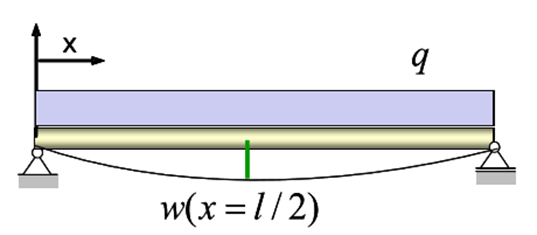
\includegraphics[width=5cm]{potential1}
	
	
\paragraph{ Inneres Potential $ \pi^{(i)} $:}
	\qquad $ V_{Biegung} = \ds\int_{0}^{l} E J\ w''\,^2 \ \dd x $  (Tilde? Dach?)
	
\paragraph{ Äußeres Potential $ \pi^{(a)} $:}
	\qquad $ V_{Kraft} = \pm \dfrac{1}{2}\ F\ w_{(f)} $
	
	Kraft und Verschiebung in verschiedene ($ + $) und gleiche ($ - $) Richtung
	
	$ V_{Streckenlast} = -\ds\int_{0}^{l} \tilde{w}_{(x)}\ q\ \dd x $
	
\subsection{Beispiel 2}

	$ V = \pi^{(i)} + \pi^{(a)} $
	
	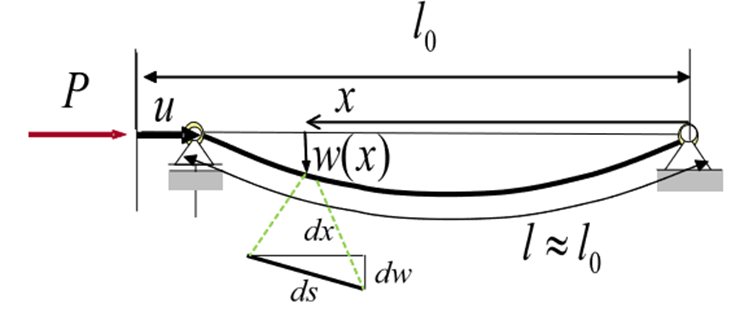
\includegraphics[width=5cm]{potential2}
	
\paragraph{ Inneres Potential $ \pi^{(i)} $}
	\qquad $ V_{Biegung}= \dfrac{1}{2} \ds \int_{0}^{l} E J\ w''\, ^2 \ \dd x $
	
\paragraph{ Äußeres Potential $ \pi^{(a)} $}
	\qquad $ V_{Kraft}  = - P u\approx - P\ \dfrac{1}{2}\ds \int_{0}^{l} w'\, ^2 \ \dd x $
	
\paragraph{	Mögliche Ansatzfunktionen:} \quad 

	Grundsätzlich kann man jegliche Funktion verwenden, aber diese soll der Biegelinie ähneln.
	
	$\rightarrow$ Potenzfunktionen: z.B. $ \varphi_{(x)}=x\ (l-x) $

	$\rightarrow$ Trigonometrische Funktionen: z.B. $ \varphi_{(x)}=\sin{\left(\dfrac{x}{l}\pi\right)} $
	
\section{Euler-Knickfälle}
	\begin{center}
		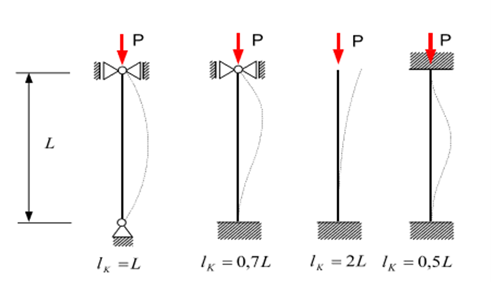
\includegraphics[width=0.7\linewidth]{euler-knick}
	\end{center}

\section{Anhang -- aus MEL2VO}
\subsection{Trägheitsmomente}
	\begin{center}
		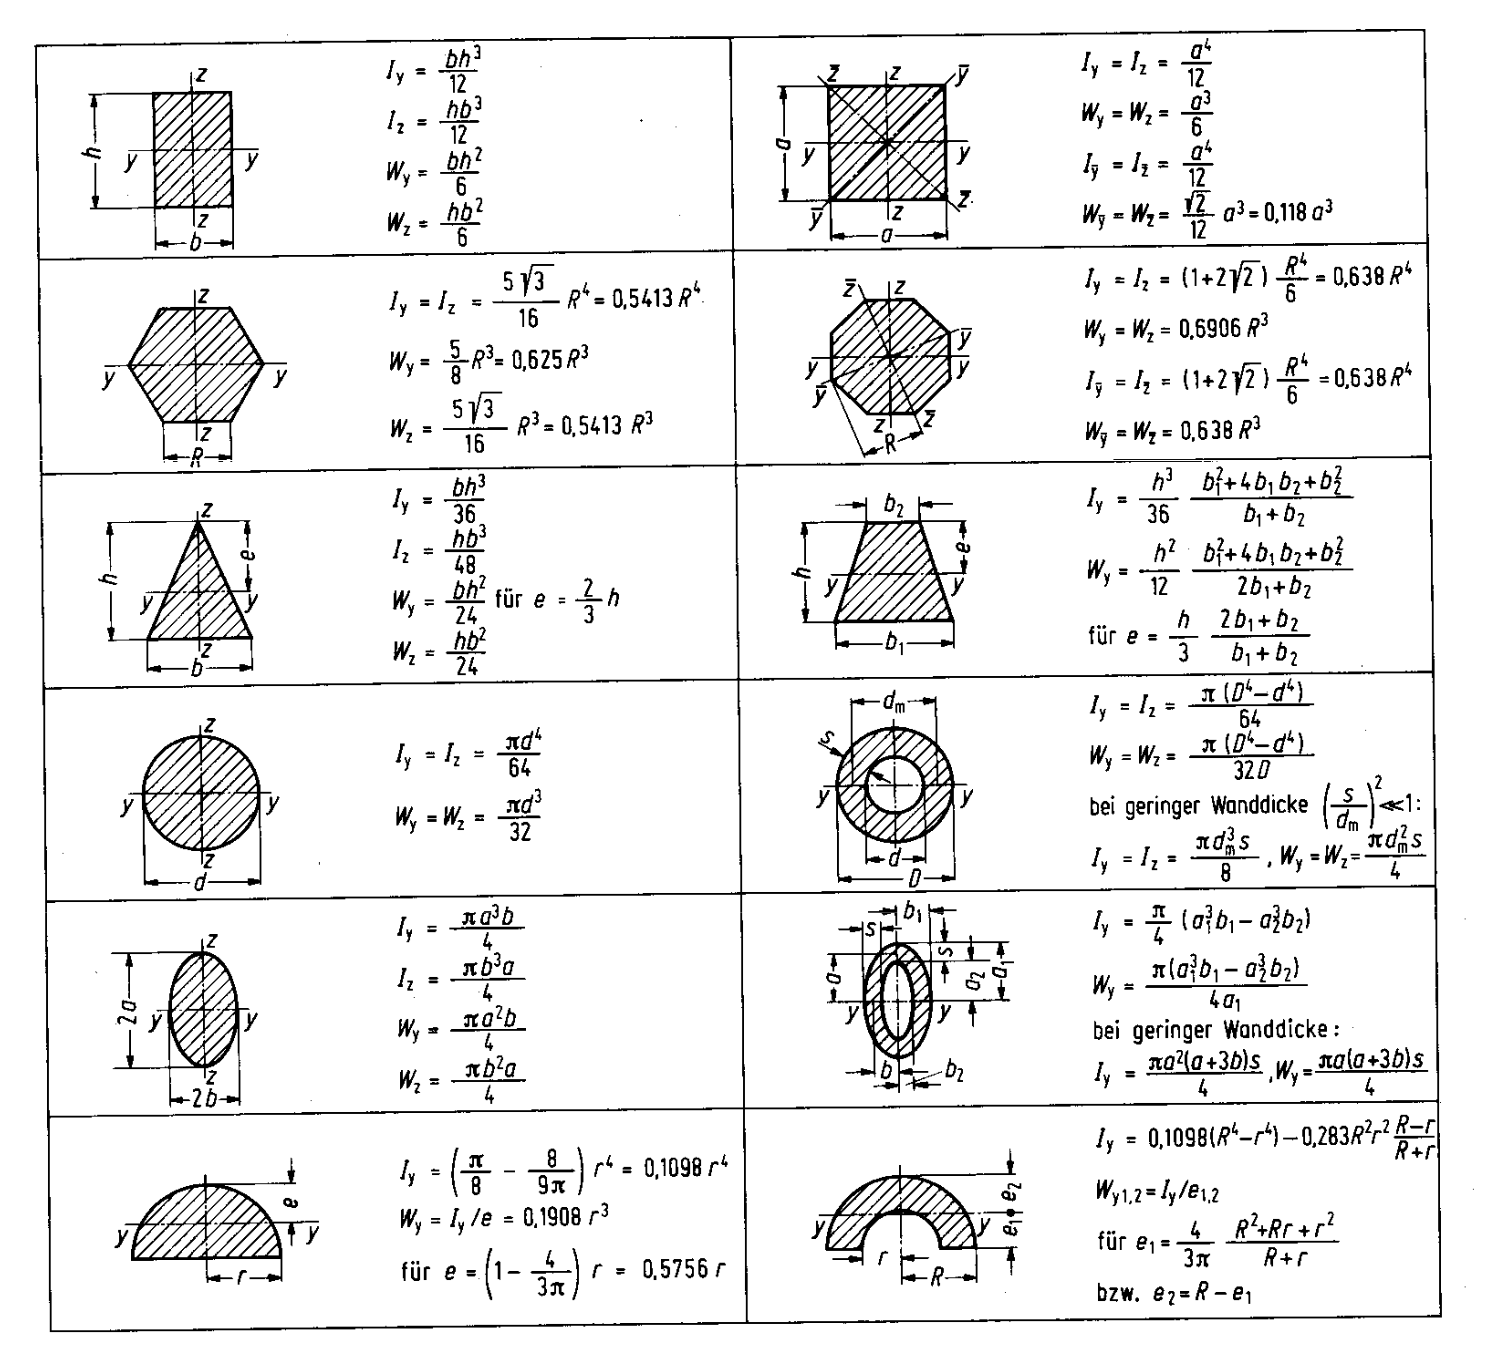
\includegraphics[width=0.8\linewidth]{Traegheit}
	\end{center}
	
\subsection{Biegelinien}
	\begin{center}
%		\includegraphics[width=0.7\linewidth]{balken-1}
		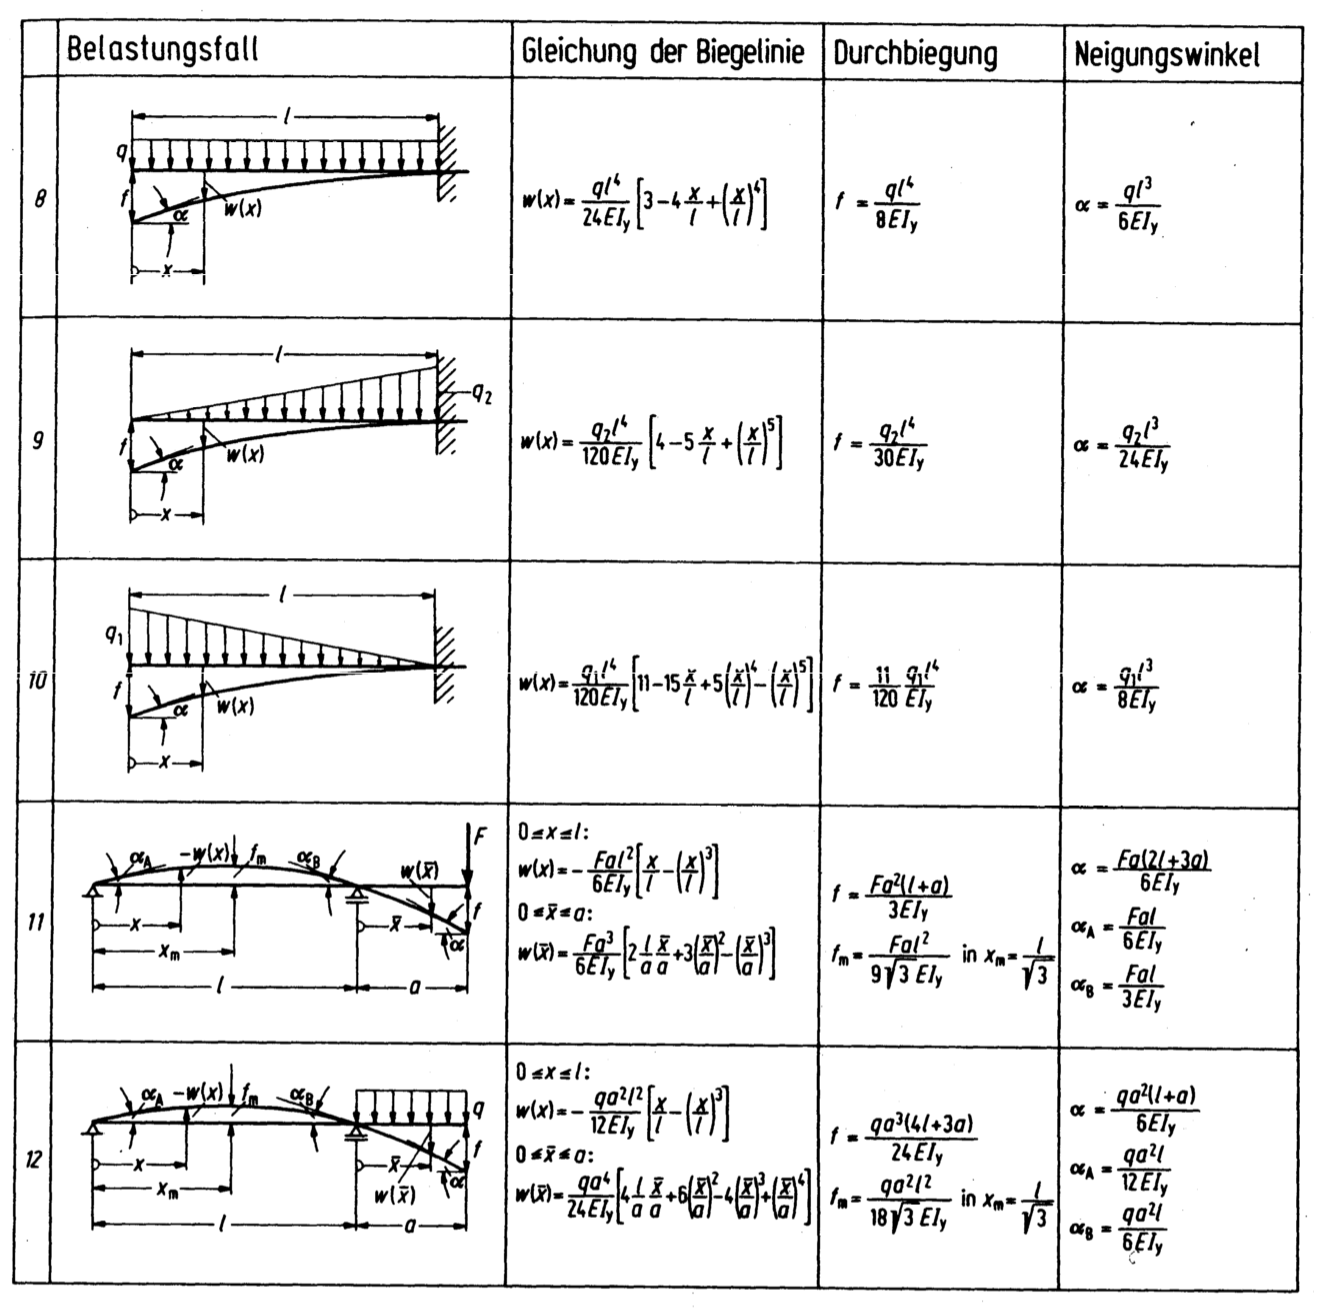
\includegraphics[width=0.7\linewidth]{balken-2}
	\end{center}